% !TeX program = xelatex
\documentclass[a4paper,10pt]{article}

% ============================================================================
% កិច្ចតែងការបង្រៀនមុខវិជ្ជាគណិតវិទ្យា ថ្នាក់ទី៨ (ម៉ោងសិក្សា ៥០ នាទី — គ្មាន LCD / ប្រើសន្លឹកកិច្ចការជាគោល)
% មេរៀនទី១៧៖ រូបធរណីមាត្រដែលមានវិមាត្របី | ម៉ោងទី៥ (១៧.៣)៖ ការគណនាមាឌនៃពីរ៉ាមីត (ទំ.២២៤–២២៥)
% វិធីសាស្ត្រ៖ 3-to-1 Prism-vs-Pyramid Contrasting Ratio + Faded Apothem-to-Altitude Pythagorean Bridge Worksheet
% ============================================================================
\usepackage[a4paper, left=0.95cm, right=0.95cm, top=0.85cm, bottom=0.92cm, footskip=0.52cm]{geometry}
\usepackage{amsmath}
\usepackage{unicode-math}
\usepackage{fontspec}
\usepackage{longtable, array, multirow, colortbl}
\usepackage[table]{xcolor}
\usepackage{enumitem}
\usepackage{pifont}
\usepackage{fancyhdr}
\usepackage{tikz}
\usetikzlibrary{calc, arrows.meta, angles, quotes, patterns, decorations.markings, babel}

\makeatletter
\let\@expl@@@mark@update@singlecol@structures@@\relax
\makeatother

% -------------------- ការស្វែងរកទីតាំងពុម្ពអក្សរដោយស្វ័យប្រវត្តិ (\NGSFindFonts) --------------------
\providecommand{\NGSFindFonts}{%
  \IfFileExists{C:/Windows/Fonts/cambria.ttc}{%
    \def\NGSSysPath{C:/Windows/Fonts/}%
    \def\NGSUserPath{C:/Users/KIT/AppData/Local/Microsoft/Windows/Fonts/}%
  }{%
    \IfFileExists{./fonts/KhmerOSsiemreap.ttf}{\def\NGSSysPath{./fonts/}\def\NGSUserPath{./fonts/}}{%
    \IfFileExists{../fonts/KhmerOSsiemreap.ttf}{\def\NGSSysPath{../fonts/}\def\NGSUserPath{../fonts/}}{%
    \IfFileExists{../../fonts/KhmerOSsiemreap.ttf}{\def\NGSSysPath{../../fonts/}\def\NGSUserPath{../../fonts/}}{%
    \IfFileExists{../../../fonts/KhmerOSsiemreap.ttf}{\def\NGSSysPath{../../../fonts/}\def\NGSUserPath{../../../fonts/}}{%
    \IfFileExists{../../../../fonts/KhmerOSsiemreap.ttf}{\def\NGSSysPath{../../../../fonts/}\def\NGSUserPath{../../../../fonts/}}{%
    \IfFileExists{../../../../../fonts/KhmerOSsiemreap.ttf}{\def\NGSSysPath{../../../../../fonts/}\def\NGSUserPath{../../../../../fonts/}}{%
    \IfFileExists{../../../../../../fonts/KhmerOSsiemreap.ttf}{\def\NGSSysPath{../../../../../../fonts/}\def\NGSUserPath{../../../../../../fonts/}}{%
      \def\NGSSysPath{../../../../../../../fonts/}\def\NGSUserPath{../../../../../../../fonts/}%
    }}}}}}}%
  }%
}
\NGSFindFonts

\setmathfont[Path={\NGSSysPath}, FontIndex=1, Scale=1.02]{cambria.ttc}
\defaultfontfeatures{Ligatures=TeX}

\setmainfont[
  Path={\NGSUserPath},
  Extension=.ttf,
  Script=Khmer,
  BoldFont={KhmerOSsiemreap},
  BoldFeatures={FakeBold=1.8},
  ItalicFont={KhmerOSsiemreap},
  ItalicFeatures={FakeSlant=0.25},
  BoldItalicFont={KhmerOSsiemreap},
  BoldItalicFeatures={FakeBold=1.8, FakeSlant=0.25}
]{KhmerOSsiemreap}

\newfontfamily\muol[
  Path={\NGSUserPath},
  Extension=.ttf,
  Script=Khmer
]{KhmerOSmuollight}

\newfontfamily\NagaBold[
  Path={\NGSUserPath},
  Extension=.ttf,
  Script=Khmer,
  ItalicFont={AKbalthom Naga Bold},
  ItalicFeatures={FakeSlant=0.22}
]{AKbalthom Naga Bold}

\newfontfamily\Tacteing[
  Path={\NGSUserPath},
  Extension=.TTF
]{TACTENG}

\newfontfamily\CalibriPage[
  Path={\NGSSysPath},
  Extension=.ttf
]{calibri}

\newfontfamily\TimesEn[
  Path={\NGSSysPath},
  Extension=.ttf,
  BoldFont={timesbd},
  ItalicFont={timesi},
  BoldItalicFont={timesbi}
]{times}

\newfontfamily\SymbolCirc[
  Path={\NGSSysPath},
  Extension=.ttf
]{cour}
\newcommand{\wcirc}{{\SymbolCirc\fontsize{10.5pt}{12pt}\selectfont o}}

\XeTeXlinebreaklocale "km"
\XeTeXlinebreakskip = 0pt plus 1pt minus 0.1pt

% -------------------- ពណ៌ និងការតុបតែង --------------------
\definecolor{darkred}{RGB}{180, 0, 0}
\definecolor{red5e}{RGB}{210, 15, 15}
\definecolor{headgray}{gray}{0.86}
\definecolor{stepgray}{gray}{0.91}
\definecolor{boxgray}{gray}{0.93}

\pagestyle{fancy}
\fancyhf{}
\renewcommand{\headrulewidth}{0pt}
\fancyfoot[R]{{\CalibriPage\fontsize{9.5pt}{11pt}\selectfont \thepage}}

\setlength{\parindent}{0pt}
\setlength{\parskip}{0pt}
\setlength{\LTpre}{2pt}
\setlength{\LTpost}{2pt}
\setlength{\tabcolsep}{4.5pt}
\arrayrulewidth=0.45pt

\newcolumntype{L}[1]{>{\raggedright\arraybackslash}p{#1}}
\newcolumntype{C}[1]{>{\centering\arraybackslash}p{#1}}

\newcommand{\en}[1]{{\TimesEn #1}}
\newcommand{\enbf}[1]{{\TimesEn\textbf{#1}}}
\newcommand{\unit}[1]{\,\text{\en{#1}}}
\newcommand{\fiveE}[1]{{\NagaBold\fontsize{9.5pt}{13pt}\selectfont\textcolor{red5e}{#1}}}
\newcommand{\timenote}[1]{\textcolor{darkred}{\textit{#1}}}
\newcommand{\khmflourish}{{\Tacteing\fontsize{17pt}{17pt}\selectfont 3}}
\newcommand{\graybox}[1]{\colorbox{boxgray}{\strut\hspace{2pt}#1\hspace{2pt}}}
\newcommand{\ditem}{\tikz[baseline=-0.5ex]\fill (0,0.42ex) -- (0.42ex,0) -- (0,-0.42ex) -- (-0.42ex,0) -- cycle;\hspace{0.3em}}
\newcommand{\cnum}[1]{{\fontsize{10.5pt}{12pt}\selectfont\ding{\numexpr181+#1\relax}}\hspace{0.2em}}
\newcommand{\cfig}[1]{\par\vspace{4pt}{\centering #1\par}\vspace{4pt}}
\newcommand{\stepheader}[1]{\multicolumn{3}{|c|}{\cellcolor{stepgray}\muol #1} \\* \noalign{\hrule height 0.4pt}}
\newcommand{\tri}[1]{\ensuremath{\triangle #1}}

\newcommand{\rightbox}[4][0.18]{%
  \draw[black, line width=0.75pt]
    ($(#3)!#1!(#2)$) -- ($($(#3)!#1!(#2)$)+($(#3)!#1!(#4)$)-(#3)$) -- ($(#3)!#1!(#4)$);
}

% ============================================================================
% រូបធរណីមាត្រ ស-ខ្មៅ (B&W Print-Safe TikZ Figures for Hour 17.5: Pyramid Volume)
% ============================================================================

% ១. កំណែកិច្ចការផ្ទះទី១៦ក (ហិបដែក ទំ.២២៩) និងរំលឹកត្រីកោណកែងខាងក្នុងពីរ៉ាមីតនិយ័ត (h, m, d)
\newcommand{\figPrereqPyrVol}{%
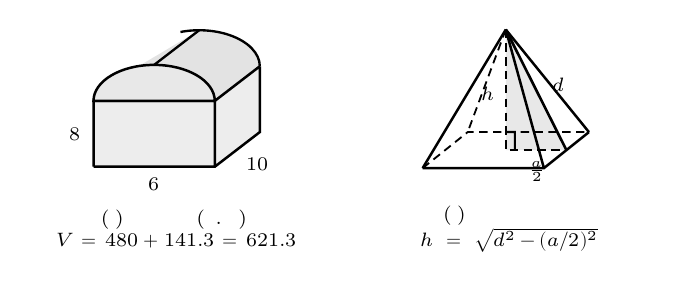
\begin{tikzpicture}[scale=0.88, every node/.style={font=\scriptsize, text=black}]
  % (ក) លំហាត់ទី១៦ក (ទំ.២២៩)៖ ហិបដែក 10x6x8 + កន្លះស៊ីឡាំង r=3, h=10
  \begin{scope}[shift={(-2.35,0)}]
    \coordinate (A) at (-1.30,-0.75);
    \coordinate (B) at (0.45,-0.75);
    \coordinate (C) at (1.10,-0.25);
    \coordinate (A1) at (-1.30,0.20);
    \coordinate (B1) at (0.45,0.20);
    \coordinate (C1) at (1.10,0.70);
    \fill[gray!14] (A) -- (B) -- (C) -- (C1) -- (B1) -- (A1) -- cycle;
    \fill[gray!22] (B1) arc (0:180:0.875 and 0.52) -- (-0.65,0.70) -- (0.225,1.22) arc (90:0:0.875 and 0.52) -- cycle;
    \draw[black, line width=0.9pt] (A) -- (B) -- (C) -- (C1) (A) -- (A1) -- (B1) -- (B) (B1) -- (C1);
    \draw[black, line width=0.9pt, fill=gray!18] (B1) arc (0:180:0.875 and 0.52) -- cycle;
    \draw[black, line width=0.85pt] (C1) arc (0:108:0.875 and 0.52);
    \draw[black, line width=0.85pt] (-0.425,0.72) -- (0.225,1.22);
    \node[below=0.5pt] at (-0.42,-0.75) {$6$};
    \node[below right=-1pt] at (0.80,-0.52) {$10$};
    \node[left=1pt] at (-1.30,-0.28) {$8$};
    \node[align=center, text width=3.55cm] at (-0.10,-1.65) {(ក) លំហាត់ទី១៦ក (ទំ.២២៩)៖\\$V = 480 + 141.3 = 621.3$};
  \end{scope}

  % (ខ) រំលឹកទំនាក់ទំនងកម្ពស់កែង h និងអាប៉ូតែម d ក្នុងពីរ៉ាមីតនិយ័ត
  \begin{scope}[shift={(2.30,-0.05)}]
    \coordinate (V) at (0,1.28);
    \coordinate (A) at (-1.20,-0.72);
    \coordinate (B) at (0.55,-0.72);
    \coordinate (C) at (1.20,-0.20);
    \coordinate (D) at (-0.55,-0.20);
    \coordinate (O) at (0,-0.46);
    \coordinate (M) at (0.875,-0.46);
    \fill[gray!18] (V) -- (O) -- (M) -- cycle;
    \draw[black, line width=0.9pt] (A) -- (B) -- (C) (V) -- (A) (V) -- (B) (V) -- (C);
    \draw[black, line width=0.65pt, densely dashed] (A) -- (D) -- (C) (V) -- (D);
    \draw[black, line width=0.85pt, densely dashed] (V) -- (O) -- (M);
    \draw[black, line width=0.95pt] (V) -- (M);
    \rightbox[0.15]{V}{O}{M}
    \node[left=0.5pt] at (0,0.35) {$h$};
    \node[below=0.5pt] at (0.45,-0.46) {$\frac{a}{2}$};
    \node[right=1pt] at (0.50,0.48) {$d$};
    \node[align=center, text width=3.65cm] at (0.05,-1.60) {(ខ) ត្រីកោណកែងខាងក្នុង៖\\$h = \sqrt{d^2 - (a/2)^2}$};
  \end{scope}
\end{tikzpicture}}

% ២. E1 Engage (លំហាត់ទី១៧ ទំ.២២៩)៖ ប៉មស្ថាបត្យកម្ម បាតការេ 5m x 5m ជញ្ជាំង 20m និងកម្ពស់សរុប 24m
\newcommand{\figEngageTower}{%
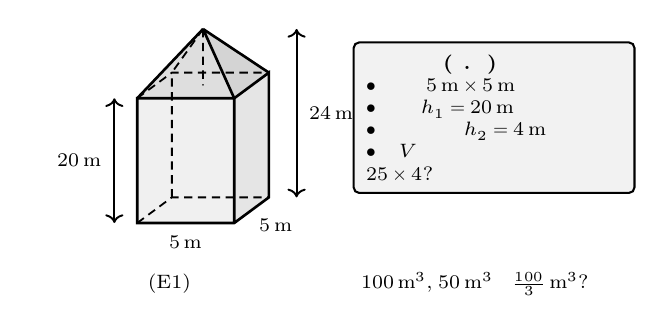
\begin{tikzpicture}[scale=0.88, every node/.style={font=\scriptsize, text=black}]
  \begin{scope}[shift={(-1.55,-0.15)}]
    \coordinate (A) at (-0.95,-1.25);
    \coordinate (B) at (0.45,-1.25);
    \coordinate (C) at (0.95,-0.88);
    \coordinate (D) at (-0.45,-0.88);
    \coordinate (A1) at (-0.95,0.55);
    \coordinate (B1) at (0.45,0.55);
    \coordinate (C1) at (0.95,0.92);
    \coordinate (D1) at (-0.45,0.92);
    \coordinate (V) at (0.0,1.55);
    \coordinate (O1) at (0.0,0.735);
    \fill[gray!12] (A) -- (B) -- (B1) -- (A1) -- cycle;
    \fill[gray!20] (B) -- (C) -- (C1) -- (B1) -- cycle;
    \fill[gray!26] (A1) -- (B1) -- (V) -- cycle;
    \fill[gray!34] (B1) -- (C1) -- (V) -- cycle;
    \draw[black, line width=0.95pt] (A) -- (B) -- (C) -- (C1) -- (B1) -- (A1) -- cycle (B) -- (B1);
    \draw[black, line width=0.95pt] (V) -- (A1) (V) -- (B1) (V) -- (C1);
    \draw[black, line width=0.65pt, densely dashed] (A) -- (D) -- (C) (D) -- (D1) (A1) -- (D1) -- (C1) (V) -- (D1) (V) -- (O1);
    \node[below=1pt] at (-0.25,-1.25) {$5\unit{m}$};
    \node[below right=-1pt] at (0.72,-1.08) {$5\unit{m}$};
    \draw[<->, line width=0.7pt] (-1.28,-1.25) -- (-1.28,0.55) node[midway, left=1pt] {$20\unit{m}$};
    \draw[<->, line width=0.7pt] (1.35,-0.88) -- (1.35,1.55) node[midway, right=1pt] {$24\unit{m}$};
  \end{scope}

  \begin{scope}[shift={(2.35,0.12)}]
    \node[draw=black, line width=0.75pt, rounded corners=2pt, fill=gray!10, inner sep=4.5pt, align=left, text width=3.25cm] at (0.30,0.0) {%
      \textbf{ប៉មលំហាត់ទី១៧ (ទំ.២២៩)៖}\\
      $\bullet$ បាតការេ $5\unit{m}\times 5\unit{m}$\\
      $\bullet$ តួប៉ម៖ $h_1 = 20\unit{m}$\\
      $\bullet$ ដំបូលពីរ៉ាមីត៖ $h_2 = 4\unit{m}$\\
      $\bullet$ តើ $V_{\text{ដំបូល}}$ ស្មើប៉ុន្មានភាគនៃប្រអប់កែង $25\times 4$?};
  \end{scope}
  \node[align=center, text width=7.3cm] at (0.20,-2.28) {បញ្ហាបំផុសគំនិត (\en{E1})៖ តើមាឌដំបូលរាងពីរ៉ាមីតស្មើនឹង $100\unit{m}^3$, $50\unit{m}^3$ ឬ $\frac{100}{3}\unit{m}^3$?};
\end{tikzpicture}}

% ៣. E2/E3 ការផ្ទេរ ៣ ដងពីពីរ៉ាមីតចូលព្រីស (ទំ.២២៤) និងលំហាត់គំរូទី 1 (បាតត្រីកោណកែង 5,6 កម្ពស់ 8)
\newcommand{\figSandAndPyrExamples}{%
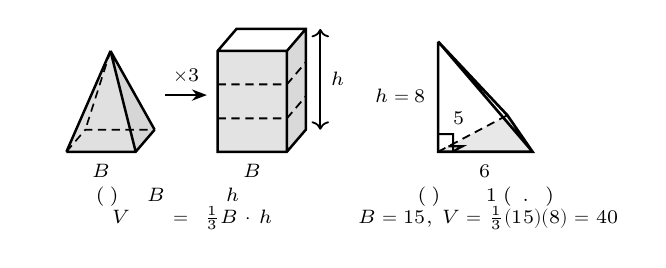
\begin{tikzpicture}[scale=0.80, every node/.style={font=\scriptsize, text=black}]
  % (ក) ពីរ៉ាមីត និង ព្រីស មានផ្ទៃបាត B និងកម្ពស់ h ដូចគ្នា => 3 ដងពេញព្រីស
  \begin{scope}[shift={(-2.55,0)}]
    % ពីរ៉ាមីត
    \coordinate (A) at (-1.55,-0.75);
    \coordinate (B) at (-0.45,-0.75);
    \coordinate (C) at (-0.15,-0.40);
    \coordinate (D) at (-1.25,-0.40);
    \coordinate (V) at (-0.85,0.85);
    \fill[gray!24] (A) -- (B) -- (V) -- cycle;
    \fill[gray!32] (B) -- (C) -- (V) -- cycle;
    \draw[black, line width=0.9pt] (A) -- (B) -- (C) (V) -- (A) (V) -- (B) (V) -- (C);
    \draw[black, line width=0.6pt, densely dashed] (A) -- (D) -- (C) (V) -- (D);
    \node[below=1pt] at (-1.00,-0.75) {$B$};

    \draw[-{Stealth[length=1.9mm]}, line width=0.85pt] (0.02,0.15) -- (0.68,0.15) node[midway, above=1pt] {$\times 3$};

    % ព្រីស (3 ស្រទាប់ស្មើៗគ្នា)
    \coordinate (P) at (0.85,-0.75);
    \coordinate (Q) at (1.95,-0.75);
    \coordinate (R) at (2.25,-0.40);
    \coordinate (P1) at (0.85,0.85);
    \coordinate (Q1) at (1.95,0.85);
    \coordinate (R1) at (2.25,1.20);
    \coordinate (S1) at (1.15,1.20);
    \fill[gray!22] (P) -- (Q) -- (Q1) -- (P1) -- cycle;
    \fill[gray!30] (Q) -- (R) -- (R1) -- (Q1) -- cycle;
    \draw[black, line width=0.65pt, densely dashed] (0.85,-0.22) -- (1.95,-0.22) -- (2.25,0.13);
    \draw[black, line width=0.65pt, densely dashed] (0.85,0.32) -- (1.95,0.32) -- (2.25,0.67);
    \draw[black, line width=0.9pt] (P) -- (Q) -- (R) -- (R1) -- (S1) -- (P1) -- cycle (P1) -- (Q1) -- (R1) (Q) -- (Q1);
    \node[below=1pt] at (1.40,-0.75) {$B$};
    \draw[<->, line width=0.65pt] (2.48,-0.40) -- (2.48,1.20) node[midway, right=0.5pt] {$h$};
    \node[align=center, text width=3.95cm] at (0.45,-1.65) {(ក) បាត $B$ និងកម្ពស់ $h$ ដូចគ្នា៖\\$V_{\text{ពីរ៉ាមីត}} = \frac{1}{3} B\cdot h$};
  \end{scope}

  % (ខ) លំហាត់គំរូទី 1 (ទំ.២២៤)៖ ពីរ៉ាមីតបាតត្រីកោណកែងជើង 5, 6 និងកម្ពស់ h=8
  \begin{scope}[shift={(2.75,-0.05)}]
    \coordinate (O) at (-0.95,-0.70);
    \coordinate (A) at (0.55,-0.70);
    \coordinate (B) at (0.15,-0.12);
    \coordinate (V) at (-0.95,1.05);
    \fill[gray!18] (O) -- (A) -- (B) -- cycle;
    \draw[black, line width=0.95pt] (V) -- (O) -- (A) -- (B) (V) -- (A) (V) -- (B);
    \draw[black, line width=0.65pt, densely dashed] (O) -- (B);
    \rightbox[0.16]{V}{O}{A}
    \rightbox[0.15]{A}{O}{B}
    \node[left=1pt] at (-0.95,0.18) {$h=8$};
    \node[below=1pt] at (-0.20,-0.70) {$6$};
    \node[above left=-1pt] at (-0.42,-0.38) {$5$};
    \node[align=center, text width=3.55cm] at (-0.15,-1.60) {(ខ) គំរូទី \en{1} (ទំ.២២៤)៖\\$B=15,\; V=\frac{1}{3}(15)(8)=40$};
  \end{scope}
\end{tikzpicture}}

% ៤. E4 ប្រតិបត្តិ ក (a=14, d=25 => h=24, V=1568) និង ប្រតិបត្តិ ខ (a=10, d=13 => h=12, V=400) ទំ.២២៥
\newcommand{\figElaboratePyrVol}{%
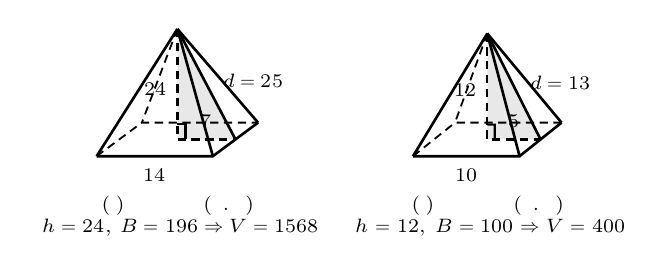
\begin{tikzpicture}[scale=0.82, every node/.style={font=\scriptsize, text=black}]
  % (១) ប្រតិបត្តិ ក (ទំ.២២៥)៖ បាតការេ a=14, អាប៉ូតែម d=25
  \begin{scope}[shift={(-2.35,0)}]
    \coordinate (V) at (0,1.25);
    \coordinate (A) at (-1.25,-0.72);
    \coordinate (B) at (0.55,-0.72);
    \coordinate (C) at (1.25,-0.20);
    \coordinate (D) at (-0.55,-0.20);
    \coordinate (O) at (0,-0.46);
    \coordinate (M) at (0.90,-0.46);
    \fill[gray!18] (V) -- (O) -- (M) -- cycle;
    \draw[black, line width=0.95pt] (A) -- (B) -- (C) (V) -- (A) (V) -- (B) (V) -- (C);
    \draw[black, line width=0.65pt, densely dashed] (A) -- (D) -- (C) (V) -- (D);
    \draw[black, line width=0.85pt, densely dashed] (V) -- (O) -- (M);
    \draw[black, line width=0.95pt] (V) -- (M);
    \rightbox[0.14]{V}{O}{M}
    \node[below=1pt] at (-0.35,-0.72) {$14$};
    \node[above=0.5pt] at (0.44,-0.46) {$7$};
    \node[left=0.5pt] at (0,0.32) {$24$};
    \node[right=1pt] at (0.52,0.45) {$d=25$};
    \node[align=center, text width=3.65cm] at (0.05,-1.65) {(១) ប្រតិបត្តិ ក (ទំ.២២៥)៖\\$h=24,\; B=196 \Rightarrow V=1568$};
  \end{scope}

  % (២) ប្រតិបត្តិ ខ (ទំ.២២៥)៖ បាតការេ a=10, អាប៉ូតែម d=13
  \begin{scope}[shift={(2.45,0)}]
    \coordinate (V) at (0,1.18);
    \coordinate (A) at (-1.15,-0.72);
    \coordinate (B) at (0.50,-0.72);
    \coordinate (C) at (1.15,-0.20);
    \coordinate (D) at (-0.50,-0.20);
    \coordinate (O) at (0,-0.46);
    \coordinate (M) at (0.825,-0.46);
    \fill[gray!18] (V) -- (O) -- (M) -- cycle;
    \draw[black, line width=0.95pt] (A) -- (B) -- (C) (V) -- (A) (V) -- (B) (V) -- (C);
    \draw[black, line width=0.65pt, densely dashed] (A) -- (D) -- (C) (V) -- (D);
    \draw[black, line width=0.85pt, densely dashed] (V) -- (O) -- (M);
    \draw[black, line width=0.95pt] (V) -- (M);
    \rightbox[0.14]{V}{O}{M}
    \node[below=1pt] at (-0.32,-0.72) {$10$};
    \node[above=0.5pt] at (0.41,-0.46) {$5$};
    \node[left=0.5pt] at (0,0.30) {$12$};
    \node[right=1pt] at (0.48,0.42) {$d=13$};
    \node[align=center, text width=3.65cm] at (0.05,-1.65) {(២) ប្រតិបត្តិ ខ (ទំ.២២៥)៖\\$h=12,\; B=100 \Rightarrow V=400$};
  \end{scope}
\end{tikzpicture}}

% ============================================================================
% ចាប់ផ្ដើមឯកសារ (Document Body)
% ============================================================================
\begin{document}
\fontsize{10pt}{15.2pt}\selectfont

% -------------------- ក្បាលកិច្ចតែងការ (Header) --------------------
\begin{center}
  {\muol\fontsize{11pt}{16pt}\selectfont ព្រះរាជាណាចក្រកម្ពុជា}\\[2pt]
  {\muol\fontsize{10pt}{15pt}\selectfont ជាតិ សាសនា ព្រះមហាក្សត្រ}\\[1pt]
  \khmflourish
\end{center}

\vspace{-26pt}
{\muol\fontsize{9.5pt}{12.8pt}\selectfont
មន្ទីរអប់រំ យុវជន និងកីឡា ខេត្តកំពង់ធំ\\
ការិយាល័យអប់រំ យុវជន និងកីឡា ស្រុកកំពង់ស្វាយ\\
អនុវិទ្យាល័យព្រះក្រសាំង}

\vspace{2pt}
\begin{center}
  {\muol\fontsize{10pt}{14.5pt}\selectfont កិច្ចតែងការបង្រៀន}
\end{center}
\vspace{1pt}

% -------------------- ព័ត៌មានទូទៅ (Metadata) --------------------
{\renewcommand{\arraystretch}{0.98}
\hspace*{4.05cm}%
\begin{tabular}{@{}l l l@{}}
  - \hspace{0.35cm} មុខវិជ្ជា & : & គណិតវិទ្យា ថ្នាក់ទី៨ \\
  - \hspace{0.35cm} ចំណងជើងមេរៀន & : & មេរៀនទី១៧ រូបធរណីមាត្រដែលមានវិមាត្របី \\
  - \hspace{0.35cm} ចំណងជើងរង & : & ១៧.៣ ការគណនាមាឌនៃពីរ៉ាមីត (ទំព័រ ២២៤--២២៥) \\
  - \hspace{0.35cm} រយៈពេល & : & ១ ម៉ោងសិក្សា (៥០ នាទី) \\
  - \hspace{0.35cm} បង្រៀនដោយ & : & ហុក ប៊ុនថែន \\
  - \hspace{0.35cm} កាលបរិច្ឆេទ & : & ថ្ងៃ\makebox[18mm]{\dotfill}\ ទី\makebox[8mm]{\dotfill}\ ខែ\makebox[18mm]{\dotfill}\ ឆ្នាំ២០២៦ \\
\end{tabular}

\vspace{3pt}

% -------------------- I. វត្ថុបំណង --------------------
\textbf{I.} {\muol វត្ថុបំណង}\\[1pt]
\hspace*{0.55cm}%
\begin{tabular}{@{}l l L{14.2cm}@{}}
  \wcirc \hspace{0.25cm} វិជ្ជាសម្បទា & : & សិស្សប្រាប់បានត្រឹមត្រូវពីទំនាក់ទំនងសមាមាត្រ $\frac{1}{3}$ រវាងមាឌពីរ៉ាមីត និងមាឌព្រីសដែលមានផ្ទៃបាត $B$ និងកម្ពស់កែង $h$ ដូចគ្នា ព្រមទាំងរូបមន្តមាឌពីរ៉ាមីត ($V = \frac{1}{3} B \cdot h$) ។ \\
  \wcirc \hspace{0.25cm} បំណិនសម្បទា & : & សិស្សបែងចែកដាច់រវាងកម្ពស់កែង $h$ និងអាប៉ូតែមមុខខាង $d$ ប្រើទ្រឹស្ដីបទពីតាករគណនា $h = \sqrt{d^2-(a/2)^2}$ រួចគណនាមាឌពីរ៉ាមីតត្រីមុខ ចតុមុខ និងសូលីតផ្សំលើសន្លឹកកិច្ចការបានត្រឹមត្រូវ ។ \\
  \wcirc \hspace{0.25cm} ចរិយាសម្បទា & : & សិស្សមានទម្លាប់ផ្ទៀងផ្ទាត់ធាតុកម្ពស់កែងមុនជំនួសក្នុងរូបមន្តមាឌ និងសហការគ្នាដោះស្រាយបញ្ហាស្ថាបត្យកម្មជាក់ស្ដែង ។ \\
\end{tabular}

\vspace{3pt}

% -------------------- II. សម្ភារៈឧបទេស --------------------
\textbf{II.} {\muol សម្ភារៈឧបទេស}\\[1pt]
\hspace*{0.55cm}$\bullet$ \hspace{0.35cm} សៀវភៅសិក្សាគោលគណិតវិទ្យាថ្នាក់ទី៨ (ទំ.២២៤--២២៥ និង ២២៨--២៣០) សន្លឹកកិច្ចការសិស្ស ស-ខ្មៅ (\en{Worksheet\_PYR\_VOL} ចំនួន ២ ទំព័រ គ្មាន \en{LCD}) ក្ដារខៀន ដីស និងបន្ទាត់ក្រិត ។

\vspace{3pt}

% -------------------- III. វិធីសាស្រ្តបង្រៀន --------------------
\textbf{III.} {\muol វិធីសាស្រ្តបង្រៀន}\\[1pt]
\hspace*{0.45cm}%
\begin{tabular}{@{}l l L{14.85cm}@{}}
  $\bullet$ \hspace{0.25cm} គោលវិធី & : & សិស្សមជ្ឈមណ្ឌល (សិក្សាតាមរយៈការបំពេញលើសន្លឹកកិច្ចការជាគោល គ្មាន \en{LCD} និងគ្មានការកាត់បិទក្រដាស) \\
  $\bullet$ \hspace{0.25cm} យុទ្ធវិធីបង្រៀន & : & ស្ថាបនានិយម គម្រូ \en{5Es} រួមបញ្ចូលការប្រៀបធៀបសមាមាត្រ ៣-ទល់-១ ព្រីស-ពីរ៉ាមីត (\en{Contrasting Ratio} $V=\frac{1}{3}Bh$) និងលំហាត់គំរូបន្ថយជំហានភ្ជាប់ពីតាករ (\en{Faded Apothem-to-Altitude Bridge}) ។ \\
\end{tabular}
}

\vspace{3pt}

% -------------------- IV. ដំណើរការបង្រៀន --------------------
\textbf{IV.} {\muol ដំណើរការបង្រៀន}

\vspace{2pt}

\renewcommand{\arraystretch}{1.15}
\begin{longtable}{|L{5.50cm}|L{7.90cm}|L{4.80cm}|}
\hline
\rowcolor{headgray}
\multicolumn{1}{|c|}{\muol សកម្មភាពគ្រូ} &
\multicolumn{1}{c|}{\muol ខ្លឹមសារមេរៀន} &
\multicolumn{1}{c|}{\muol សកម្មភាពសិស្ស} \\
\hline
\endfirsthead

\hline
\rowcolor{headgray}
\multicolumn{1}{|c|}{\muol សកម្មភាពគ្រូ} &
\multicolumn{1}{c|}{\muol ខ្លឹមសារមេរៀន} &
\multicolumn{1}{c|}{\muol សកម្មភាពសិស្ស} \\
\hline
\endhead

\hline
\endfoot

\hline
\endlastfoot

% ==================== ជំហានទី១ (2 min) ====================
\stepheader{ជំហានទី១ (រដ្ឋបាលថ្នាក់)}
$\bullet$ ពិនិត្យវត្តមាន សណ្ដាប់ធ្នាប់ អនាម័យ និងចែកសន្លឹកកិច្ចការ \en{Worksheet\_PYR\_VOL} ដល់សិស្សគ្រប់គូ \timenote{(2 min)}
&
$\bullet$ រដ្ឋបាលថ្នាក់ និងការត្រៀមសៀវភៅគោល បន្ទាត់ក្រិត និងសន្លឹកកិច្ចការសិស្ស
&
$\circ$ ប្រធានថ្នាក់រាយការណ៍វត្តមាន\par\vspace{2pt}
$\circ$ ទទួលសន្លឹកកិច្ចការ និងត្រៀមឧបករណ៍ \\[3pt]
\hline

% ==================== ជំហានទី២ (9 min: ≤3 + 3 + E1 3) ====================
\stepheader{ជំហានទី២ (កិច្ចការផ្ទះ + រំលឹកមេរៀនចាស់ + ទំនាក់ទំនងមេរៀនថ្មី)}
\timenote{(កំណែកិច្ចការផ្ទះ $\le 3\text{ min}$)}\par\vspace{1pt}
$\bullet$ ផ្ទៀងផ្ទាត់ចម្លើយលំហាត់ទី៨ ក,ខ,ឃ (ទំ.២២៨) និងទី១៦ក (ទំ.២២៩ ហិបដែក) លើក្ដារខៀនយ៉ាងរហ័ស
&
\textbf{កំណែកិច្ចការផ្ទះ (ទំ.២២៨ ទី៨ក,ខ,ឃ និងទំ.២២៩ ទី១៦ក)៖}\par\vspace{1pt}
$1.$ \textbf{ទី៨៖} (ក) $14\times 10\times 8 = \mathbf{1120}$;\; (ខ) $10\times 15\times 10 = \mathbf{1500}$;\; (ឃ) $3.14(10^2)(10) = \mathbf{3140}$ ។\par\vspace{1pt}
$2.$ \textbf{ទី១៦ក (ហិបដែក)៖} $V = (10\times 6\times 8) + \frac{1}{2}(3.14)(3^2)(10) = 480 + 141.3 = \graybox{$621.3$}$ ។
&
$\circ$ ផ្ទៀងផ្ទាត់និងកែកំណែលំហាត់ទី៨ក,ខ,ឃ និងទី១៦ក ក្នុងសៀវភៅ \\[3pt]

\timenote{(រំលឹកមេរៀនចាស់ 3 min)}\par\vspace{1pt}
$\bullet$ សួរ៖ «តើមាឌនៃព្រីសស្មើនឹងអ្វី? ហើយក្នុងពីរ៉ាមីតនិយ័តបាតការេជ្រុង $a$ និងអាប៉ូតែមមុខខាង $d$ តើយើងរកកម្ពស់កែង $h$ តាមទ្រឹស្ដីបទអ្វី?»
&
\textbf{រំលឹករូបមន្តមាឌព្រីស និងត្រីកោណកែងខាងក្នុងពីរ៉ាមីត៖}\par\vspace{1pt}
\ditem មាឌព្រីស៖ $V_{\text{ព្រីស}} = B \cdot h$ ។\par\vspace{1pt}
\ditem តាមពីតាករក្នុងពីរ៉ាមីតនិយ័តបាតការេជ្រុង $a$៖ $h = \sqrt{d^2 - \left(\frac{a}{2}\right)^2}$ ។
&
$\circ$ ឆ្លើយរំលឹករូបមន្ត $V=B\cdot h$ និងទំនាក់ទំនង $h = \sqrt{d^2-(a/2)^2}$ \\[3pt]

& \cfig{\figPrereqPyrVol} & \\[3pt]

\fiveE{E1 - Engage} \timenote{(3 min)}\par\vspace{1.5pt}
$\bullet$ បង្ហាញបញ្ហាប៉មស្ថាបត្យកម្មលើ \textbf{បេសកកម្មទី១ (\en{E1})} (ដកស្រង់ពីលំហាត់ទី១៧ ទំ.២២៩)៖\par\vspace{1pt}
\hspace*{0.3em}-- «ប៉មមួយមានបាតការេជ្រុង $5\unit{m}$ តួជញ្ជាំងឈររាងប្រអប់កែងកម្ពស់ $20\unit{m}$ និងដំបូលកំពូលរាងពីរ៉ាមីតដែលធ្វើឱ្យកម្ពស់សរុបស្មើ $24\unit{m}$ ($h_{\text{ដំបូល}} = 4\unit{m}$) ។ តើមាឌដំបូលពីរ៉ាមីតស្មើនឹង $100\unit{m}^3$, $50\unit{m}^3$ ឬ $\frac{100}{3}\unit{m}^3$?»
&
\textbf{១៧.៣ ការគណនាមាឌនៃពីរ៉ាមីត}\par\vspace{1.5pt}
\ditem \textbf{បញ្ហាបំផុសគំនិត (\en{E1 - POE})៖} ពីរ៉ាមីតរួមតូចទៅរកកំពូលតែមួយ! តើមាឌរបស់វាស្មើប៉ុន្មានភាគនៃមាឌព្រីសដែលមានបាត $B$ និងកម្ពស់កែង $h$ ដូចគ្នា?
&
$\circ$ អានបេសកកម្មទី១ ពិភាក្សាជាដៃគូ និងគូសធីកទស្សន៍ទាយ (\en{Predict}) \\[3pt]

& \cfig{\figEngageTower} & \\[3pt]
\hline

% ==================== ជំហានទី៣ (17 min: E2 11 + E3 6) ====================
\stepheader{ជំហានទី៣ (ខ្លឹមសារមេរៀនថ្មី)}
\fiveE{E2 - Explore} \timenote{(11 min: 5 min)}\par\vspace{1pt}
$\bullet$ ឱ្យសិស្សធ្វើជាដៃគូលើ \textbf{ផ្នែកទី១ (ក) ការប្រៀបធៀបព្រីស-ពីរ៉ាមីត និងការបំបែកគូបជា $6$ ពីរ៉ាមីត} តាមទំ.២២៤
&
\textbf{សកម្មភាពរុករកទី១ (សមាមាត្រ ៣-ទល់-១ និងការបំបែកគូប)៖}\par\vspace{1pt}
$1.$ ចាក់ខ្សាច់ពេញពីរ៉ាមីតចូលក្នុងព្រីសដែលមានបាត $B$ និងកម្ពស់ $h$ ស្មើគ្នា ត្រូវចាក់ \textbf{៣ ដង} ទើបពេញព្រីស $\Rightarrow 3 V_{\text{ពីរ៉ាមីត}} = B\cdot h$ ។
&
$\circ$ សង្កេតដ្យាក្រាមផ្ទេរ ៣ ដង ទាញបាន $3V_{\text{ពីរ៉ាមីត}} = B\cdot h$ \\[3pt]

$\bullet$ ណែនាំឱ្យគូសិស្សពិនិត្យការបំបែកគូបទ្រនុង $a$ ត្រង់ផ្ចិត $O$ បានពីរ៉ាមីតប៉ុនគ្នាចំនួន $6$
&
$2.$ ផ្ទៀងផ្ទាត់តាមគូបទ្រនុង $a$ (មាឌ $a^3$)៖ អង្កត់ទ្រូងទាំង ៤ បំបែកគូបជា \textbf{ពីរ៉ាមីតប៉ុនគ្នាចំនួន $6$} ដែលមួយៗមានបាត $B=a^2$ និងកម្ពស់ $h=\frac{a}{2}$ ៖\par\vspace{1pt}
\hspace*{0.3em}$V = \dfrac{a^3}{6} = \dfrac{1}{3} a^2 \cdot \left(\dfrac{a}{2}\right) \Rightarrow$ \graybox{$V = \dfrac{1}{3} B \cdot h$} ។
&
$\circ$ ផ្ទៀងផ្ទាត់តាមការបំបែកគូបជា $6$ ពីរ៉ាមីត ទាញបាន $V = \frac{1}{3}B\cdot h$ \\[3pt]

\timenote{(E2 ទី២៖ លំហាត់គំរូទី \en{1} និងទី \en{2} ទំ.២២៤ — 6 min)}\par\vspace{1.5pt}
$\bullet$ ដឹកនាំសិស្សបំពេញ \textbf{ផ្នែកទី១ (ខ) គំរូទី \en{1}} (ពីរ៉ាមីតបាតត្រីកោណកែង) តាមសៀវភៅទំ.២២៤
&
\textbf{សកម្មភាពរុករកទី២ — លំហាត់គំរូទី \en{1} និងទី \en{2} (ទំ.២២៤)៖}\par\vspace{1.5pt}
$\bullet$ \textbf{គំរូទី \en{1} (បាតត្រីកោណកែងជើង $5, 6$; កម្ពស់កែង $h = 8$)៖}\par\vspace{1pt}
\hspace*{0.2em}$B = \frac{1}{2}\times 5\times 6 = 15 \Rightarrow V = \frac{1}{3}\times 15\times 8 = \mathbf{40}$ ឯកតាមាឌ ។
&
$\circ$ គណនាគំរូទី \en{1} បាន $B=15,\; V=40$ \\[3pt]

$\bullet$ បន្តឱ្យសិស្សបំពេញ \textbf{គំរូទី \en{2}} (ពីរ៉ាមីតបាតចតុ.កែង $7\times 5$ កម្ពស់ $6$)
&
$\bullet$ \textbf{គំរូទី \en{2} (បាតចតុ.កែង $7\times 5$; កម្ពស់កែង $h = 6$)៖}\par\vspace{1pt}
\hspace*{0.2em}$B = 7\times 5 = 35 \Rightarrow V = \frac{1}{3}\times 35\times 6 = \graybox{$70$}$ ឯកតាមាឌ ។
&
$\circ$ គណនាគំរូទី \en{2} បាន $B=35,\; V=70$ \\[3pt]

& \cfig{\figSandAndPyrExamples} & \\[3pt]

\fiveE{E3 - Explain} \timenote{(6 min)}\par\vspace{1.5pt}
$\bullet$ ហៅតំណាងគូបង្ហាញ រួចគ្រូសង្ខេបរូបមន្តមាឌពីរ៉ាមីត (ប្រអប់ទំ.២២៤) ឱ្យសិស្សបំពេញ \textbf{ផ្នែកទី២}
&
\textbf{រូបមន្តមាឌនៃពីរ៉ាមីត (ទំ.២២៤)៖}\par\vspace{1.5pt}
$\bullet$ មាឌនៃពីរ៉ាមីតស្មើនឹងមួយភាគបីនៃផលគុណរវាងផ្ទៃក្រឡាបាត ($B$) និងកម្ពស់កែង ($h$)៖ \graybox{$V = \dfrac{1}{3} B \cdot h$} ។
&
$\circ$ តំណាងគូឡើងបកស្រាយ\par\vspace{2pt}
$\circ$ បំពេញប្រអប់រូបមន្តក្នុងផ្នែកទី២ \\[3pt]

$\bullet$ បំបែកអន្ទាក់យល់ច្រឡំដ៏ធំរវាង \textbf{កម្ពស់កែង $h$} និង \textbf{អាប៉ូតែមមុខខាង $d$} ព្រមទាំងធនាគារហេតុផល \cnum{1}--\cnum{4}
&
\textbf{ការបែងចែក $h$ និង $d$ ព្រមទាំងធនាគារហេតុផល៖}\par\vspace{1.5pt}
$\bullet$ \textbf{ប្រយ័ត្ន៖} $S_l = \frac{1}{2}P\cdot d$ ប្រើ \textbf{អាប៉ូតែមទ្រេត $d$} ឯមាឌ $V = \frac{1}{3}B\cdot h$ ប្រើ \textbf{កម្ពស់កែង $h$}!\par\vspace{1pt}
$\bullet$ \cnum{1} $B =$ ផ្ទៃបាតពហុកោណ \;\textbar\; \cnum{2} $h = \sqrt{d^2-(a/2)^2}$ ជាកម្ពស់កែង \;\textbar\; \cnum{3} $V = \frac{1}{3}B\cdot h$ \;\textbar\; \cnum{4} សូលីតផ្សំ៖ $V = V_{\text{ព្រីស}} + V_{\text{ពីរ៉ាមីត}}$ ។
&
$\circ$ កត់ចំណាំភាពខុសគ្នារវាង $h$ និង $d$ ព្រមទាំងធនាគារហេតុផល \cnum{1}--\cnum{4} \\[3pt]
\hline

% ==================== ជំហានទី៤ (20 min: E4 10 + E5 10) ====================
\stepheader{ជំហានទី៤ (ពង្រីកចំណេះដឹង និងវាយតម្លៃ)}
\fiveE{E4 - Elaborate} \timenote{(10 min: 5 min)}\par\vspace{1pt}
$\bullet$ ឱ្យសិស្សធ្វើជាដៃគូលើ \textbf{ផ្នែកទី៣ (ក) ប្រតិបត្តិ ក (ទំ.២២៥)} សម្រាប់ពីរ៉ាមីតនិយ័តបាតការេជ្រុង $14$ និងអាប៉ូតែម $d=25$
&
\textbf{៣.ក ប្រតិបត្តិ ក (ទំ.២២៥ — ពីរ៉ាមីតបាតការេជ្រុង $a=14,\; d=25$)៖}\par\vspace{1.5pt}
$\bullet$ កន្លះជ្រុងបាត $\frac{a}{2} = 7 \Rightarrow$ កម្ពស់កែង $h = \sqrt{25^2 - 7^2} = \sqrt{576} = \mathbf{24}$ \cnum{2} ។\par\vspace{1pt}
$\bullet$ ផ្ទៃបាត $B = 14^2 = 196$ \cnum{1} $\Rightarrow V = \frac{1}{3}(196)(24) = 196\times 8 = \graybox{$1568$}$ \cnum{3} ។
&
$\circ$ ប្រើពីតាកររក $h=24$ រួចគណនា $B=196$ និងមាឌ $V=1568$ \\[3pt]

\timenote{(E4 ទី២៖ ប្រតិបត្តិ ខ ទំ.២២៥ — 5 min)}\par\vspace{1.5pt}
$\bullet$ ឱ្យសិស្សដោះស្រាយ \textbf{ផ្នែកទី៣ (ខ) ប្រតិបត្តិ ខ (ទំ.២២៥)} ដោយខ្លួនឯង រួចសួរ \en{EIA Looking-Back}៖ «ហេតុអ្វីមិនយក $\frac{1}{3}\times 100\times 13$?»
&
\textbf{៣.ខ ប្រតិបត្តិ ខ (ទំ.២២៥ — ពីរ៉ាមីតបាតការេជ្រុង $a=10,\; d=13$)៖}\par\vspace{1.5pt}
$\bullet$ កន្លះជ្រុងបាត $\frac{a}{2} = 5 \Rightarrow$ កម្ពស់កែង $h = \sqrt{13^2 - 5^2} = \sqrt{144} = \mathbf{12}$ \cnum{2} ។\par\vspace{1pt}
$\bullet$ ផ្ទៃបាត $B = 10^2 = 100 \Rightarrow V = \frac{1}{3}\times 100\times 12 = \graybox{$400$}$ ឯកតាមាឌ \cnum{3} ។
&
$\circ$ រក $h=12, B=100$ និងគណនាបាន $V=400$ ដោយមិនច្រឡំយក $d=13$ \\[3pt]

& \cfig{\figElaboratePyrVol} & \\[3pt]

\fiveE{E5 - Evaluate} \timenote{(10 min: 6 min)}\par\vspace{1pt}
$\bullet$ ឱ្យសិស្សធ្វើ \textbf{ផ្នែកទី៤ (ក) បកស្រាយបេសកកម្ម \en{E1} (លំហាត់ទី១៧ ទំ.២២៩ — ប៉មស្ថាបត្យកម្ម)} ដោយឯករាជ្យលើសន្លឹកកិច្ចការ
&
\textbf{រង្វាយតម្លៃទី១ — បកស្រាយបេសកកម្ម \en{E1} (លំហាត់ទី១៧ ទំ.២២៩)៖}\par\vspace{1.5pt}
$\bullet$ ផ្ទៃបាតការេ៖ $B = 5\times 5 = 25\unit{m}^2$;\; មាឌតួប៉ម៖ $V_1 = 25\times 20 = \mathbf{500\unit{m}^3}$ ។
&
$\circ$ គណនាផ្ទៃបាត $B=25\unit{m}^2$ និងមាឌតួប៉ម $V_1=500\unit{m}^3$ \\[3pt]

$\bullet$ ដើរពិនិត្យការគណនាមាឌដំបូលពីរ៉ាមីត $V_2$ និងមាឌប៉មសរុប $V = V_1 + V_2$
&
$\bullet$ កម្ពស់ដំបូលពីរ៉ាមីត៖ $h_2 = 24 - 20 = 4\unit{m} \Rightarrow V_2 = \frac{1}{3}(25)(4) = \mathbf{33\frac{1}{3}\unit{m}^3}$ ។\par\vspace{1pt}
$\Rightarrow$ មាឌសរុបនៃប៉ម៖ $V = 500 + 33\frac{1}{3} = \graybox{$533\frac{1}{3}\unit{m}^3 \approx 533.33\unit{m}^3$}$ \cnum{4} ។
&
$\circ$ គណនា $V_2=33\frac{1}{3}\unit{m}^3$ និងមាឌប៉មសរុប $533\frac{1}{3}\unit{m}^3$ \\[3pt]

\timenote{(E5 ទី២៖ \en{Exit Check} — 4 min)}\par\vspace{1.5pt}
$\bullet$ ឱ្យសិស្សគូសវង់ \textbf{\en{Exit Check} ៣ សំណួរ (ផ្នែកទី៤ ខ)} រួមទាំងលំហាត់ទី១០ក (ទំ.២២៨) និងលើកម្រាមដៃបង្ហាញចម្លើយ
&
\textbf{រង្វាយតម្លៃទី២ — \en{Exit Check}៖}\par\vspace{1.5pt}
$\bullet$ សំណួរទី១ ($V_{\text{ព្រីស}}=90\unit{cm}^3$) $\to$ \textbf{ខ} ($30\unit{cm}^3$); សំណួរទី២ (ទី១០ក ទំ.២២៨៖ $B=100\unit{cm}^2, VO=12\unit{cm}$) $\to$ \textbf{ក} ($400\unit{cm}^3$); សំណួរទី៣ ($a=6, d=5, h=4$) $\to$ \textbf{គ} ($\frac{1}{3}(36)(4)=48\unit{cm}^3$) ។
&
$\circ$ គូសវង់ \en{Exit Check} និងលើកម្រាមដៃបង្ហាញចម្លើយ \\[3pt]
\hline

% ==================== ជំហានទី៥ (≤2 min) ====================
\stepheader{ជំហានទី៥ (កិច្ចការផ្ទះ + បណ្ដាំផ្ញើ)}
\timenote{(ចំណាយពេល $\le 2\text{ min}$)}\par\vspace{1.5pt}
$\bullet$ ដាក់កិច្ចការផ្ទះ (ទំ.២២៨ លំហាត់ទី៨ង និងទំ.២៣០ លំហាត់ទី២១) និងណែនាំអានមេរៀនមាឌកោន
&
\centerline{\muol កិច្ចការផ្ទះ}\par\vspace{2pt}
$1.$ \textbf{លំហាត់ទី៨ ង (ទំ.២២៨)៖} គណនាមាឌសូលីតផ្សំពីគូបទ្រនុង $20\unit{ft}$ និងពីរ៉ាមីតកំពូលដែលមានកម្ពស់ $15\unit{ft}$ ។\par\vspace{1.5pt}
$2.$ \textbf{លំហាត់ទី២១ (ទំ.២៣០)៖} គណនាមាឌពីរ៉ាមីតចតុមុខនិយ័តដែលមានអង្កត់ទ្រូងបាតការេស្មើ $10\unit{dm}$ និងទ្រនុងខាងស្មើ $13\unit{dm}$ (ណែនាំ៖ $B = \frac{10^2}{2} = 50\unit{dm}^2$ និងកន្លះអង្កត់ទ្រូងបាត $= 5\unit{dm}$) ។\par\vspace{1.5pt}
$3.$ \textbf{អានមេរៀនបន្ទាប់៖} ១៧.៤ ការគណនាមាឌនៃកោន (ទំ.២២៥--២២៦) ។
&
$\circ$ កត់ត្រាលំហាត់ទី៨ង និងទី២១ ព្រមទាំងអានមេរៀនមាឌកោន\par\vspace{2pt}
$\circ$ ជម្រាបលាលោកគ្រូ \\[3pt]
\end{longtable}

% -------------------- កាលបរិច្ឆេទ និងហត្ថលេខា --------------------
\vspace{10pt}
\hfill
\begin{minipage}{9.8cm}
  {\centering
    ថ្ងៃ\makebox[16mm]{\dotfill}\ ខែ\makebox[18mm]{\dotfill}\ ឆ្នាំមមី អដ្ឋស័ក ពុទ្ធសករាជ ២៥៧០\\[2pt]
    កំពង់ស្វាយ, ថ្ងៃទី\makebox[10mm]{\dotfill}\ ខែ\makebox[18mm]{\dotfill}\ ឆ្នាំ២០២៦\\[3pt]
    {\muol គ្រូបង្រៀន}\par}
  \vspace{32pt}
  \hfill{\muol ហុក ប៊ុនថែន}\hspace*{1.4cm}
\end{minipage}

\end{document}
